\documentclass{article}
\usepackage[utf8]{inputenc}
\usepackage{hyperref}
\usepackage[letterpaper, portrait, margin=1in]{geometry}
\usepackage{enumitem}
\usepackage{amsmath}
\usepackage{booktabs}
\usepackage{graphicx}

\usepackage{hyperref}
\hypersetup{
colorlinks=true,
    linkcolor=black,
    filecolor=black,      
    urlcolor=blue,
    citecolor=black,
}
\usepackage{natbib}

\usepackage{titlesec}
  
\title{ECON 7103 Homework 3}
\author{Yifan Liu (yliu3494)}
\date{Spring 2023}
  
\begin{document}
  
\maketitle


\noindent
(a) Show that $ln(y_i) = \alpha + ln(\delta) d_i + \gamma ln(z_i) + \eta_i$
\bigskip
\\
Given $y_i = e^{\alpha} \delta^{d_i} z_i^{\gamma} e^{\eta_i}$,
\\
natural log transformation on both sides leads to
\\
$ln(y_i) = \alpha ln(e) + d_i ln(\delta)  + \gamma ln(z_i) + \eta_i ln(e)$
\\
$ln(y_i) = \alpha + ln(\delta) d_i + \gamma ln(z_i) + \eta_i$
\bigskip
\bigskip

\noindent
(b) The intuitive interpretation of $\delta$:
\bigskip
\\
The households receiving the retrofits are expected to have $\delta$ units less of electricity consumption than households without retrofits, holding all other variables constant.
\smallskip
\\
To be more specific, when $d_i$ changes from 0 (indicating no retrofits) to 1 (indicating retrofits), $ln(y_i)$ changes by $ln(\delta)$, meaning that $y_i$ changes by $\delta$ units. 
\bigskip
\bigskip

\noindent
(c) Show that $\frac{\Delta y_i}{\Delta d_i} = \frac{\delta - 1}{\delta^{d_i}}  y_i$
\bigskip
\\
LHS = $\frac{\Delta y_i}{\Delta d_i} = \frac{e^{\alpha} \delta^{(d_i = 1)} z_i^{\gamma} e^{\eta_i} - e^{\alpha} \delta^{(d_i = 0)} z_i^{\gamma} e^{\eta_i}}{(d_i = 1) - (d_i = 0)}$
\bigskip
\\
= $e^{\alpha} \delta z_i^{\gamma} e^{\eta_i} - e^{\alpha}  z_i^{\gamma} e^{\eta_i}$
\bigskip
\\
= $(\delta - 1) e^{\alpha} z_i^{\gamma} e^{\eta_i}$
\bigskip
\\
= $\frac{(\delta - 1) e^{\alpha} z_i^{\gamma} e^{\eta_i} \delta^{d_i}}{\delta^{d_i}}$ 
\bigskip
\\
= $\frac{\delta - 1}{\delta^{d_i}}  y_i$
= RHS
\bigskip
\bigskip

\noindent
The intuitive interpretation of $\frac{\Delta y_i}{\Delta d_i}$ the average marginal effects of the retrofit program. 
\bigskip
\\
In other words, for each household, it refers to the change in electricity consumption resulting from participating in the energy-efficiency retrofit program, compared with the benchmark of not receiving the retrofit. 
\bigskip
\bigskip

\noindent
(d) Show that $\frac{\partial y_i}{\partial z_i} = \gamma \frac{y_i}{z_i}$ 
\bigskip
\\
LHS = $\frac{\partial y_i}{\partial z_i}$
\bigskip
\\
= $\gamma e^{\alpha} \delta^{d_i} z_i^{\gamma - 1} e^{\eta_i}$
\bigskip
\\
= $\gamma \frac{e^{\alpha} \delta^{d_i} z_i^{\gamma} e^{\eta_i}}{z_i}$
\bigskip
\\
= $\gamma \frac{y_i}{z_i}$ = RHS
\bigskip
\bigskip

\noindent
The intuitive interpretation of $\frac{\partial y_i}{\partial z_i}$ is the average marginal effects of the square feet of the home.
\bigskip
\\
In other words, for each household, it refers to the change in electricity consumption associated with the change in the square feet of the home.
\bigskip
\bigskip

\noindent
(e) Regression results
\begin{table}[hbt!]
    \centering
    \begin{tabular}{lll}
\toprule
{} & Coefficient Estimates & Average Marginal Effect Estimates \\
{} &                  (CI) &                              (CI) \\
\midrule
retrofit &                   0.9 &                              -114 \\
         &          (0.89, 0.92) &                 (-193.07, -57.47) \\
sqft     &                  0.89 &                              0.63 \\
         &          (0.88, 0.91) &                      (0.49, 0.79) \\
temp     &                  0.28 &                              4.02 \\
         &          (0.04, 0.52) &                      (1.97, 6.91) \\
\bottomrule
\end{tabular}

    \caption{The coefficient estimate and the marginal effect estimate}
    \label{tab:table_e}
\end{table}


\bigskip
\bigskip
\noindent
(f)  Graph the average marginal effects
\begin{figure}[hbt!]
    \centering
    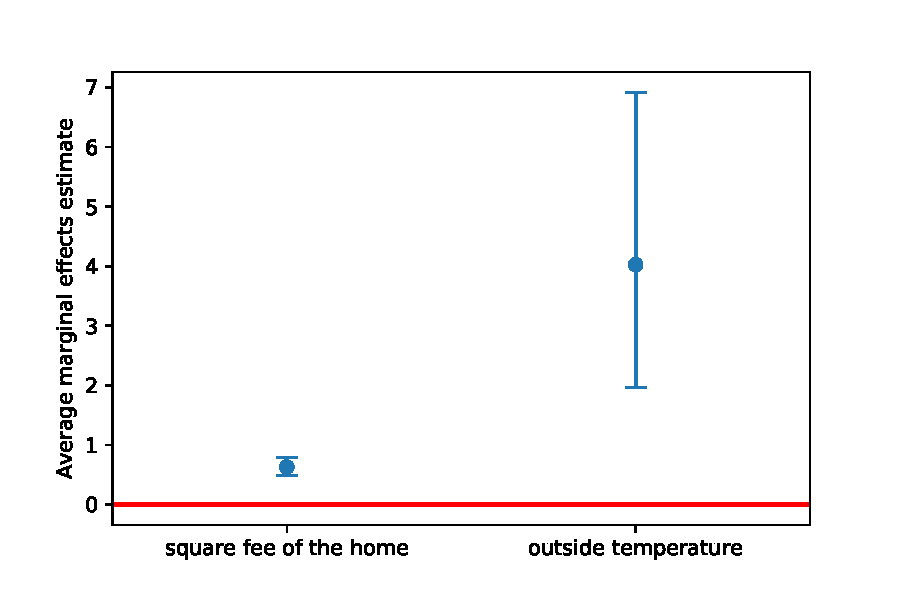
\includegraphics[scale = 0.7]{bar_f.pdf}
    \caption{Average marginal effects of outdoor temperature and square feet of the home with their bootstrapped confidence intervals}
    \label{fig:bar_f}
\end{figure}
\bigskip
\\
From Figure 1 we can see that the average marginal effect of the outdoor temperature is larger than that of the square feet of the home. The variance of the average marginal effect of the outdoor temperature is larger too. 



\end{document}